\section{The Focus on the Problem}

\subsection{The History}

As one can see from the following list:
\begin{itemize}
\setlength{\itemsep}{0.05\baselineskip}
    \item Journals of the Continental Congress - Articles of War, 20 September, 1776 . \cite{ArticlesOfWar1775:online}\\
    \textit{An example: Section XIII, Article 12: Whatsoever officer or soldier shall misbehave himself before the enemy, or shamefully abandon any post committed to his charge, or shall speak words inducing others to do the like, shall super death.}
    \item General Orders No. 100 : The Lieber Code, Instructions for the government of armies of the US in the field, 24 April 1863. \cite{LiberCode1863:online}\\
    \textit{An example: Article 16: Military necessity does not admit of cruelty - that is, the infliction of suffering for the sake of suffering or for revenge, nor of maiming or wounding except in fight, nor of torture to extort confessions. It does not admit of the use of poison in any way, nor of the wanton devastation of a district. It admits of deception, but disclaims acts of perfidy; and, in general, military necessity does not include any act of hostility which makes the return to peace unnecessarily difficult. }
    \item Amelioration of the Condition of the Wounded on the Field of Battle (Red Cross Convention), First Geneva Convention; 22 August, 1864. \cite{1stGenevaConvention1864:online}\\
    \textit{An example: Article 1: Ambulances and military hospitals shall be acknowledged to be neuter, and, as such, shall be protected and respected by belligerents so long as any sick or wounded may be therein.\\
    Such neutrality shall cease if the ambulances or hospitals should be held by a military force. }
    \item Final Act of the Diplomatic Conference of Geneva, 12 August 1949. \cite{FinalGenevaConvention1949:online}\\
    \textit{An example: ARTICLE 34: During the last two world wars, hostages were imprisoned, often put in solitary confinement, deported and in many cases executed without previous warning or trial.\\
    The International Committee of the Red Cross considered that the prohibition of such practices, which are based on contempt for the principle of individual responsibility for breaches of the law, must be one of the essential elements in the new Convention.}
\end{itemize}
Changes to the conduct of warfare by nations, and on a global scale, has been put in place. These conducts have also been updated to also contain articles enforcing practices , as Prof. Yves Sandoz writes, "for the protection of persons at the mercy of or in the hands of their enemy" and practices to prevent "Use of certain conventional weapons which may be deemed to be excessively injurious or to have indiscriminate effects" \cite{ConventionalWeapons1980:online}\\

\iffalse
\begin{chronology}[3]{1991}{2012}{\linewidth}[17cm]
\event{\decimaldate{}{9}{1991}}{{“The Coward’s War: Landmines in Cambodia" report}}
\event{\decimaldate{}{10}{1992}}{{Six \gls{ngo}s meet and agree to coordinate campaigning efforts}}
\event{\decimaldate{}{5}{1993}}{{The ICBL holds its First International \gls{ngo} Conference on Landmines}}
\event{\decimaldate{}{3}{1994}}{{UNICEF Director Jim Grant calls for a landmine ban}}
\event{\decimaldate{}{3}{1995}}{{Belgium becomes the first country to pass a national law banning landmine}}
\event{\decimaldate{}{10}{1996}}{{Canada hosts a conference in Ottawa attended by 75 governments, the ICBL and international agencies}}
%\event{\decimaldate{}{10}{1997}}{{The ICBL and Jody Williams are awarded the Nobel Peace Prize for their crucial roles}}
\event{\decimaldate{}{11}{1997}}{{A total of 122 nations sign the Mine Ban Treaty in Ottawa, Canada}}
\event{\decimaldate{}{6}{1998}}{{The ICBL creates the Landmine Monitor initiative to verify nations’ compliance with the Mine Ban Treaty}}
\event{\decimaldate{}{3}{1999}}{{Mine Ban Treaty enters into force on 1 March 1999, becoming binding international law}}
\event{\decimaldate{}{7}{2000}}{{Mauritania becomes the 100Th country to ratify the Mine Ban Treaty}}
\event{\decimaldate{}{3}{2003}}{{All States Parties with stockpiles to destroy complete their obligations deadline.}}
\event{\decimaldate{}{9}{2004}}{{An international symposium on the challenges of achieving a mine-free world is held in Ottawa.}}
\event{\decimaldate{}{10}{2012}}{{The ICBL celebrates its 20Th anniversary}}
\end{chronology}
\fi

\begin{figure}[ht!]
    \begin{chronology}[3]{1991}{2013}{\linewidth}[17cm]
\event{\decimaldate{}{}{1991}}{{\gls{ngo}s supporting a ban on landmines begin collaborating.}}
\event{\decimaldate{}{}{1992}}{{International campaign to ban landmines is established.}}
\event{\decimaldate{}{}{1993}}{{First international meeting of NGOs held in London.}}
\event{\decimaldate{}{}{1994}}{{ICRC declares its support for a ban on antipersonnel landmines.}}
\event{\decimaldate{}{}{1995}}{{First national law banning antipersonnel mines.}}
\event{\decimaldate{}{}{1996}}{{Canada launches the Ottawa process to ban landmines.}}
%\event{\decimaldate{}{10}{1997}}{{The ICBL and Jody Williams are awarded the Nobel Peace Prize for their crucial roles}}
\event{\decimaldate{}{}{1997}}{{Mine Band Treaty adopted  an.d opened for signature.}}
\event{\decimaldate{}{}{1998}}{{Mine Ban Treaty's 40Th ratification is secured in record time.}}
\event{\decimaldate{}{}{1999}}{{The Mine Ban Treaty becomes international law.}}
\event{\decimaldate{}{}{2000}}{{Mine Ban Treaty reaches 100 states parties.}}
\event{\decimaldate{}{}{2002}}{{Affected states continue to join the Mine Ban Treaty.}}
\event{\decimaldate{}{}{2003}}{{First Stockpile destruction - Deadlines are met.}}
\event{\decimaldate{}{}{2004}}{{First Review conference of the Mine Ban Treaty.}}
event{\decimaldate{}{}{2005}}{{Use of landmines decreases.}}
\event{\decimaldate{}{}{2006}}{{Act Now to implement the Mine Ban Treaty.}}
\event{\decimaldate{}{}{2007}}{{A Success in Progress: The Mine Ban Treaty's first decade.}}
\event{\decimaldate{}{}{2009}}{{“Mission Possible” – Mine Ban Treaty's second review conference.}}
\event{\decimaldate{}{}{2010}}{{The United States consults on its landmine policy review.}}
\event{\decimaldate{}{10}{2012}}{{The ICBL-CMC celebrates its 20Th anniversary.}}
\end{chronology}
\caption{Timeline of the international campaign to ban landmines \cite{TimelineICBL:online}}
\label{fig:Timeline of the international campaign to ban landmines}
\end{figure}

\noindent Looking through the figure \ref{fig:Timeline of the international campaign to ban landmines} above, the \gls{ngo}s started in 1991 to address the issues with landmines with a report, Coward’s War - Land Mines in Cambodia, where in the report it was stated that the landmines resulted in devastating medical, social and psychological effects for Cambodia. \cite{Cambodia1991:online}. As one part in warfare, landmines have been used, but they state problems for the local civilians in the contaminated areas, see chapter \ref{chap:casualties}. And up until 1999 there was not any international law, enforced by the union of countries, to prevent countries at war to use landmines, but in 1999 the Mine Ban Treaty, also known as the Ottawa Treaty, became an international binding law that from 2000 was enforced by 100 countries, also referred to, on figure \ref{fig:Timeline of the international campaign to ban landmines}, as state parties. While this report was written, the Mine Ban Treaty is still being monitored by the \gls{icbl}. Publishing yearly the Landmine Monitor report. \cite{LandmineMonitor2019}


\subsection{UN's Involvement}

In 1997 the United Nations formed an initiative know as \gls{unmas} (Abbreviated \gls{unmas}), \gls{unmas} leads, coordinates and implements UN's demining efforts and to eliminate explosive hazards, according to UN the initiative has already saved lives and protected the livelihood of many civilians in areas of Libya, Colombia, Somalia, and many more
Further more \gls{unmas} provides some guidelines on how to give support to the survivors of landmines, although the support is mainly the responsibility of each state, but \gls{unmas} does say that all survivors should be treated fairly, which means the survivors should be treated neutrally and without discrimination

\newpage

\subsection{The Financial Aid for the Cause}

According to the \gls{icbl} \gls{lm} 2018. The total support for Mine Action in 2018 was US\$699.5. The funding for Min Action, mentioned in chapter \ref{chap:Introduction}, goes into different sections within the umbrella term Mine Action. The \gls{icbl} has set the sections as in the following figure \ref{fig:contributions_by_thematic_sector_2018}:

\begin{figure}[ht]
  \centering
  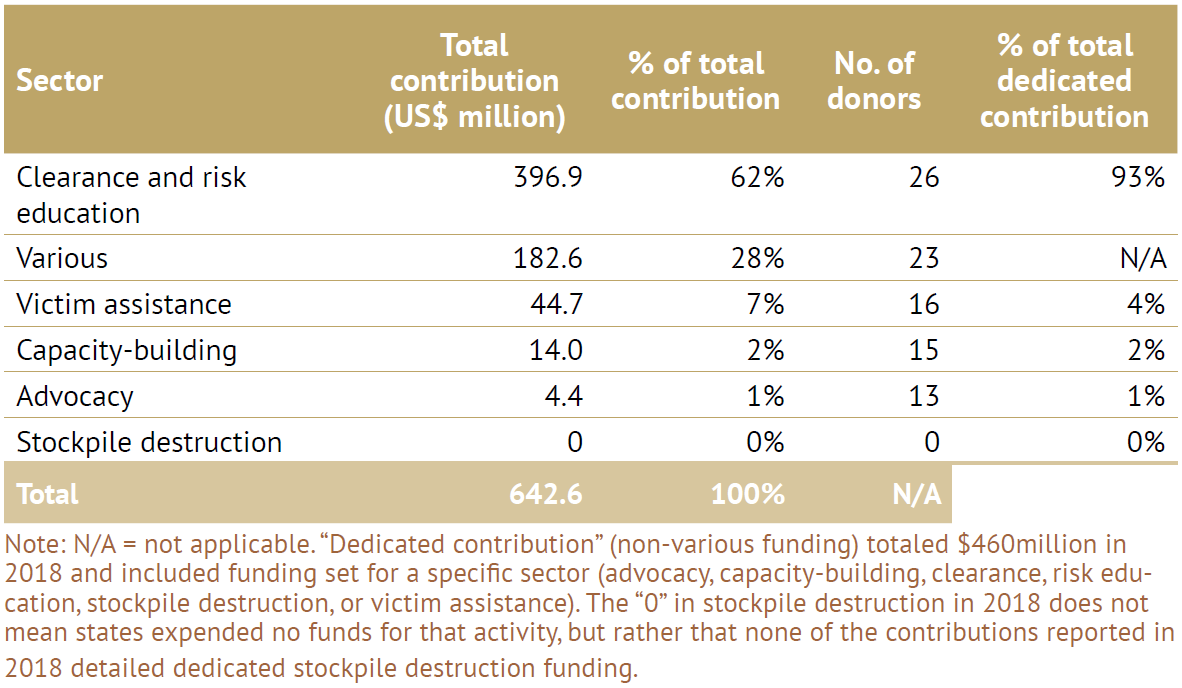
\includegraphics[width=0.6\linewidth]{00 - Images/contributions_by_thematic_sector_2018.png}
  \caption{Contributions by thematic sector 2018 \cite{LandmineMonitor2019}}
  \label{fig:contributions_by_thematic_sector_2018}
\end{figure}

The descriptiveness follows, mostly taken from \gls{lm}: 
\begin{itemize}
\setlength{\itemsep}{0.05\baselineskip}
    \item Clearance and risk education\\
    \textit{\textbf{Clearance} – Tasks or actions to ensure the removal and/or the destruction of all mine and ERW hazards from a specified area to a specified depth\\
    \textbf{Mine/\gls{erw} risk education} – Activities which seek to reduce the risk of injury from mines and  ERW by awareness-raising and  promoting behavioral  change, including public information dissemination, education and training, and community mine action liaison}
    \item Various\\
    \textit{Expenses that are not, or have not been, categorized into the other areas.}
    \item Victim assistance\\
    \textit{Victim assistance includes, but is not limited to, data collection and needs assessment, emergency and continuing medical care, physical rehabilitation, psychological support and social inclusion, economic inclusion, and laws and public policies to ensure the full and equal integration and participation of survivors, their families, and communities in society.}
    \item Capacity-building\\
    \textit{At the individual and organizational level, the focus is on increasing the availability of information and participation of underprivileged, underserved, or impoverished members of society. The purpose of these activities is to give voice and status to previously underrepresented populations. The mechanisms for building individual capacity are often leadership training, political activism, and community development. Programs that build awareness are also often highlighted. For nonprofit organizations and communities, capacity is built through technical assistance, organizational development, and interorganizational collaboration \cite{EB:capacity-building}.}
    \item Advocacy\\
    \textit{The most important assets at the disposal of advocacy networks are information and communication. Information is deployed to change actors’ perceptions and preferences and ultimately their behaviors. Information is invariably a critical component of conventional and unconventional campaign tactics, including education and capacity building, public relations, petitions, lobbying, and product or producer boycotts\cite{EB:advocacy-networking}.}
    \item Stockpile destruction\\
    \textit{Destruction of stockpiled anti-personnel mines}
\end{itemize}